\XtoCBlock{MinMaxPeriodic}
\label{block:MinMaxPeriodic}
\begin{figure}[H]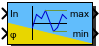
\includegraphics{MinMaxPeriodic}\end{figure} 

\begin{XtoCtabular}{Inports}
In & Input signal\tabularnewline
\hline
phi & Angle signal\tabularnewline
\hline
\end{XtoCtabular}


\begin{XtoCtabular}{Outports}
max & Maximum of input signal\tabularnewline
\hline
min & Minimum of input signal\tabularnewline
\hline
\end{XtoCtabular}

\subsubsection*{Description:}
Outputs the minimum and maximum of the input signal over one period of the (angle) signal phi.

% include optional documentation file
\InputIfFileExists{\XcHomePath/Library/Filter/Doc/MinMaxPeriodic_Info.tex}{\vspace{1ex}}{}

\subsubsection*{Implementations:}
\begin{tabular}{l l}
\textbf{FiP16} & 16 Bit Fixed Point Implementation\tabularnewline
\textbf{FiP32} & 32 Bit Fixed Point Implementation\tabularnewline
\textbf{Float32} & 32 Bit Floating Point Implementation\tabularnewline
\textbf{Float64} & 64 Bit Floating Point Implementation\tabularnewline
\end{tabular}

\XtoCImplementation{FiP16}
\nopagebreak[0]

16 Bit Fixed Point Implementation

\begin{XtoCtabular}{Inports Data Type}
In & int16\tabularnewline
\hline
phi & int16\tabularnewline
\hline
\end{XtoCtabular}

\begin{XtoCtabular}{Outports Data Type}
max & int16\tabularnewline
\hline
min & int16\tabularnewline
\hline
\end{XtoCtabular}

\ifdefined \AddTestReports
\InputIfFileExists{\XcHomePath/Library/Filter/Doc/Test-Results/Test_MinMaxPeriodic_FiP16.tex}{}{}
\fi
\XtoCImplementation{FiP32}
\nopagebreak[0]

32 Bit Fixed Point Implementation

\begin{XtoCtabular}{Inports Data Type}
In & int32\tabularnewline
\hline
phi & int32\tabularnewline
\hline
\end{XtoCtabular}

\begin{XtoCtabular}{Outports Data Type}
max & int32\tabularnewline
\hline
min & int32\tabularnewline
\hline
\end{XtoCtabular}

\ifdefined \AddTestReports
\InputIfFileExists{\XcHomePath/Library/Filter/Doc/Test-Results/Test_MinMaxPeriodic_FiP32.tex}{}{}
\fi
\XtoCImplementation{Float32}
\nopagebreak[0]

32 Bit Floating Point Implementation

\begin{XtoCtabular}{Inports Data Type}
In & float32\tabularnewline
\hline
phi & float32\tabularnewline
\hline
\end{XtoCtabular}

\begin{XtoCtabular}{Outports Data Type}
max & float32\tabularnewline
\hline
min & float32\tabularnewline
\hline
\end{XtoCtabular}

\ifdefined \AddTestReports
\InputIfFileExists{\XcHomePath/Library/Filter/Doc/Test-Results/Test_MinMaxPeriodic_Float32.tex}{}{}
\fi
\XtoCImplementation{Float64}
\nopagebreak[0]

64 Bit Floating Point Implementation

\begin{XtoCtabular}{Inports Data Type}
In & float64\tabularnewline
\hline
phi & float64\tabularnewline
\hline
\end{XtoCtabular}

\begin{XtoCtabular}{Outports Data Type}
max & float64\tabularnewline
\hline
min & float64\tabularnewline
\hline
\end{XtoCtabular}

\ifdefined \AddTestReports
\InputIfFileExists{\XcHomePath/Library/Filter/Doc/Test-Results/Test_MinMaxPeriodic_Float64.tex}{}{}
\fi
